\subsection{Polarization Wobble : Sinuous Antenna}

\subsubsection{Description of Effect}
A sinuous antenna is part of a class of planar antenna geometries called log-periodic antennas due to a log-periodic winding of the antenna arms. The benefit of log periodic antennas is the fact that their properties such as impedance, and beam properties stay consistent over a wide bandwidth and repeat every $ln(\tau)$ where $\tau$ is the characteristic length scale over which the antenna arm pattern repeats. The maximum and minimum bandwidth of these antennas are in theory just set by their inner and outer radii. One characteristic of log periodic antennas that is problematic for polarization measurements of the CMB is polarization wobble. This is a rotation of the polarization axis that oscillates between a maximum and minimum value every $\ln(\tau)$. Within the class of log-periodic antennas the sinuous antenna has the lowest amount of polarization wobble and the amount of antenna wobble is set by $\tau$: lower $\tau$ corresponds to smaller max to min deviation in polarization axis. A detailed studies of the PB2 sinuous antennas can be found in \cite{Obrient2008},\cite{Edwards2012}.
\subsubsection{Associated Systematics}
Polarization wobble is primarily a problem because is creates cross polarization or Q -> U leakage. Systematics from PB2 antennas as well as detectors and lenslets can be found in some details in Toki's thesis \cite{TokiThesis}.

\paragraph{Plan to model and/or measure:}
Minimizing $\tau$ minimizes cross polarization but smaller $\tau$ also sets the required linewidths of your traces. For POLARBEAR a $\tau$ of 1.3 was chosen to minimize $\tau$ but still allow for fabricate-able trace widths. To further null the effect of cross polarization from polarization wobble a 4 pixel differencing scheme has been proposed \cite{TokiThesis},\cite{TokiMemo1},\cite{TokiMemo2}, which will return Q and U values independent of the polarization wobble angle. This procedure requires two sets of two pixels each (A and B as shown in fig. 1) with each set having one antenna with one linear polarization oriented at 0 degrees and the second pixel rotated by 45 degrees. The polarization wobble angle is denoted as $\phi(\nu)$, the angle of incident light is $\theta(\nu)$, the detectors efficiency is $\eta(\nu)$, and the electric field amplitude is $E(\nu)$. This setup is depicted in figure 1. The steps to extract Q and U values for the 4 pixels with the dependence on $\phi(\nu)$ removed is described below. First (3) show the relative power on the the 90 and 45 pixels of the A and B sets.
\begin{figure}
\centering
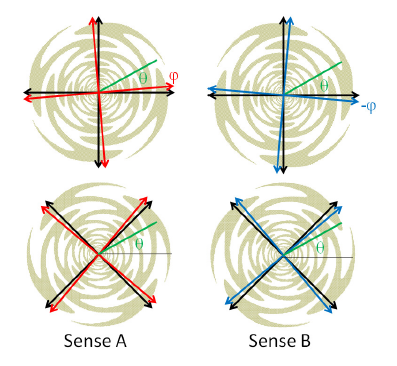
\includegraphics[width=2.5in]{4pixelremovewobble.png}
\caption{Illustration of 4 pixels with polarization wobble. Each set A and B have both a 0 \& 90 degree orientation antenna and a 45 \& -45 degree orientation pixel. $\theta$ is the polarization angle of incoming light, and $\phi$ is the polarization wobble angle.}
\label{4pixelwobbleremoval}
\end{figure}
\begin{equation}
\begin{split}
&P_{A0} = \int \eta(\nu)[E(\nu)cos(\theta(\nu)-\phi(\nu))]^2 d\nu \\
&P_{A90} = \int \eta(\nu)[E(\nu)sin(\theta(\nu)-\phi(\nu))]^2 d\nu \\
&P_{A45} = \int \eta(\nu)[E(\nu)cos(\frac{\pi}{4}-\theta(\nu)+\phi(\nu))]^2 d\nu \\
&P_{A-45} = \int \eta(\nu)[E(\nu)sin(\frac{\pi}{4}-\theta(\nu)+\phi(\nu))]^2 d\nu \\
&P_{B0} = \int \eta(\nu)[E(\nu)cos(\theta(\nu)+\phi(\nu))]^2 d\nu \\
&P_{B90} = \int \eta(\nu)[E(\nu)sin(\theta(\nu)+\phi(\nu))]^2 d\nu \\
&P_{B45} = \int \eta(\nu)[E(\nu)cos(\frac{\pi}{4}-\theta(\nu)-\phi(\nu))]^2 d\nu \\
&P_{B-45} = \int \eta(\nu)[E(\nu)sin(\frac{\pi}{4}-\theta(\nu)-\phi(\nu))]^2 d\nu
\end{split}
\end{equation}
We then assume that $\theta$ is constant across our spectral band and difference opposite orientation detectors to extract Q and U:
\begin{equation}
\begin{split}
&Q_A= P_{A0}-P_{A90}=\int \eta(\nu)E^2(\nu)cos[2(\theta-\phi(\nu))]d\nu \\
&Q_B = P_{B0}-P_{B90}=\int \eta(\nu)E^2(\nu)cos[2(\theta+\phi(\nu))] d\nu \\
&U_A = P_{A45}-P_{A-45}\int \eta(\nu)E^2(\nu)sin[2(\theta-\phi(\nu))] d\nu \\
&U_B =  P_{B45}-P_{B-45}\int \eta(\nu)E^2(\nu)sin[2(\theta+\phi(\nu))] d\nu \\
\end{split}
\end{equation}
Using trig angle sum formula (4) can be expanded to (5) 
\begin{equation}
\begin{split}
&Q_A= \int \eta(\nu)E^2(\nu)[cos(2(\theta)cos(2\phi(\nu))+sin(2(\theta)sin(2\phi(\nu))]d\nu \\
&Q_B = \int \eta(\nu)E^2(\nu)[cos(2(\theta)cos(2\phi(\nu))-sin(2(\theta)sin(2\phi(\nu))]d\nu \\
&U_A = \int \eta(\nu)E^2(\nu)[sin(2(\theta)cos(2\phi(\nu))-cos(2(\theta)sin(2\phi(\nu))]d\nu \\
&U_B =  \int \eta(\nu)E^2(\nu)[sin(2(\theta)cos(2\phi(\nu))+cos(2(\theta)sin(2\phi(\nu))]d\nu \\
\end{split}
\end{equation}
Taking linear combinations of the above Q's and U's we can define new Q's and U's as shown in (6)
\begin{equation}
\begin{split}
&Q_1=\frac{Q_A+Q_B}{2}= cos(2\theta)\int \eta(\nu)E^2(\nu)cos(2\phi(\nu))d\nu \\
&Q_2 = \frac{U_B-Q_A}{2}= cos(2\theta)\int \eta(\nu)E^2(\nu)sin(2\phi(\nu))d\nu \\
&U_1 = \frac{Q_A-Q_B}{2}= sin(2\theta)\int \eta(\nu)E^2(\nu)sin(2\phi(\nu))d\nu \\
&U_2 =  frac{U_A+U_B}{2}= sin(2\theta)\int \eta(\nu)E^2(\nu)cos(2\phi(\nu))d\nu \\
\end{split}
\end{equation}
From (6) you can then extract $\theta$ by (7)
\begin{equation}
\theta=\frac{1}{2}tan^{-1}\frac{U_{1,2}}{Q_{2,1}}
\end{equation}
E-field amplitude can also be attained from these pixels by (8)
\begin{equation}
E^2=\frac{P_{A0}+P_{A90}}{\int\eta(\nu)d\nu}=\frac{P_{A45}+P_{A-45}}{\int\eta(\nu)d\nu}=\frac{P_{B0}+P_{B90}}{\int\eta(\nu)d\nu}=\frac{P_{B45}+P_{B-45}}{\int\eta(\nu)d\nu}
\end{equation}
Where $\eta(\nu)$ is measured using an FTS.

\paragraph{Uncertainty/Range:}
\textbf{To be filled}

\paragraph{Parameterization:}
\textbf{To be filled}

%\subsubsection{References}
%\begin{itemize}
%\item O'Brient, B. \textit{et.al.}, "Sinuous-Antenna coupled TES bolometers for Cosmic Microwave Background
%Polarimetry," LTD13 Proceedings (2009).
%\item Edwards, J.M. \textit{et.al.}, "Dual-Polarized Sinuous Antennas on Extended
%Hemispherical Silicon Lenses," IEEE Trans Antennas and Propagation, Vol 60, No 9 (2012).
%\item Suzuki, A. "Lenslet Coupled Sinuous Antenna Systematic Study", Berkeley Memo (2015). - Ask for this, its not published.
%\item Suzuki, A. "Sinuous Antenna Wobble Cancellation", Berkeley Memo (2012). - Ask for this, its not published.
%\item O'Brient, B. \textit{et.al.}, "Sinuous Antennas for Cosmic Microwave Background
%Polarimetry," SPIE, Vol 7020 70201H-1 (2008).
%\item Suzuki, A. "Multichroic Bolometric Detector Architecture for Cosmic Microwave Background Polarimetry Experiments," Berkeley Dissertation (2013).
%\end{itemize} 
